%\documentclass[11pt,english]{article}
%
%% Set page margins correctly
%\usepackage{geometry}
%%\geometry{letterpaper,top=0.5in,left=0.5in,bottom=0.5in,top=0.5in,headsep=6pt,footskip=18pt}
%\geometry{letterpaper,top=0.5in,left=0.5in,bottom=0.5in,top=0.5in,headsep=6pt,footskip=18pt}
%
%% Use fancy header style
%\usepackage{fancyhdr}
%\pagestyle{fancy}
%\renewcommand{\headrulewidth}{0.75pt}
%\renewcommand{\footrulewidth}{0.75pt}
%\lhead{\footnotesize Principal Investigator/Program Director (Last, First, Middle): }
%\rhead{Yushkevich, Paul A.} \lfoot{\footnotesize PHS 398/2590 (Rev. 04/06)} \rfoot{\footnotesize
%\textbf Continuation Format Page} \cfoot{\footnotesize Page \underline{~~\thepage~~}}
%
%% Use pslatex fonts
%\usepackage{pslatex}
%\renewcommand{\familydefault}{\sfdefault}
%\renewcommand{\baselinestretch}{.9}
%




% START JUNK
\documentclass[11pt,english]{article}

% Set page margins correctly
\usepackage{geometry}
\usepackage{url}
\geometry{letterpaper,top=1.0in,left=1.0in,bottom=1.0in,top=1.0in,headsep=6pt,footskip=18pt}

\usepackage{lscape}
\usepackage[round,semicolon,authoryear,]{natbib}

% Use fancy header style
\usepackage{fancyhdr}
\pagestyle{empty}
\renewcommand{\headrulewidth}{0.75pt}
\renewcommand{\footrulewidth}{0.75pt}
%\lhead{\footnotesize Principal Investigator/Program Director (Last, First, Middle): }
%\rhead{Gee, James C.} \lfoot{\footnotesize PHS398 (06/07)} \rfoot{\footnotesize
%\textbf Continuation Format Page} \cfoot{\footnotesize Page \underline{~~\thepage~~}}

\usepackage{setspace}
\usepackage{listings}
\usepackage{float}


\floatstyle{plain}
\newfloat{command}{thp}{lop}
\floatname{command}{Command}

\doublespacing

% Use pslatex fonts
%\usepackage[T1]{fontenc}
%\usepackage{mathptmx}


% END JUNK

% All other packages
\usepackage{boxedminipage}
\usepackage{graphicx}
\usepackage{amsmath,amsfonts}
\usepackage{babel}
\usepackage{enumerate}
%\usepackage{dsfont}
\usepackage{longtable}
\usepackage{multirow}
\usepackage{sectsty}
\usepackage[compact]{titlesec}
\usepackage[usenames]{color}
\usepackage{ulem}
\usepackage{multirow,booktabs,ctable,array}

%GATHER{../../../shared/bibtex/biblio.bib}
%GATHER{../../../shared/bibtex/brainmri.bib}
%GATHER{../../../shared/bibtex/registration.bib}
\graphicspath{{./Figures/}
                          }

%\DeclareMathOperator*{\argmax}{arg\,max}
\newcommand{\argmax}{\operatornamewithlimits{argmax}}
\newcommand{\argmin}{\operatornamewithlimits{argmin}}

\long\def\symbolfootnote[#1]#2{\begingroup%
\def\thefootnote{\fnsymbol{footnote}}\footnote[#1]{#2}\endgroup}

    \usepackage{color}

    \definecolor{listcomment}{rgb}{0.0,0.5,0.0}
    \definecolor{listkeyword}{rgb}{0.0,0.0,0.5}
    \definecolor{listnumbers}{gray}{0.65}
    \definecolor{listlightgray}{gray}{0.955}
    \definecolor{listwhite}{gray}{1.0}

\newcommand{\lstsetcpp}
{
\lstset{frame = tb,
        framerule = 0.25pt,
        float,
        fontadjust,
        backgroundcolor={\color{listlightgray}},
        basicstyle = {\ttfamily\scriptsize},
        keywordstyle = {\ttfamily\color{listkeyword}\textbf},
        identifierstyle = {\ttfamily},
        commentstyle = {\ttfamily\color{listcomment}\textit},
        stringstyle = {\ttfamily},
        showstringspaces = false,
        showtabs = false,
        numbers = none,
        numbersep = 6pt,
       numberstyle={\ttfamily\color{listnumbers}},
        tabsize = 2,
        language=[ANSI]C++,
        floatplacement=!h,
        caption={\small \baselineskip 12pt Atropos short command line menu which is invoked using the `{\ttfamily -h}' option. 
        The expanded menu, which provides additional details regarding the possible parameters and usage 
        options, is elicited using the `{\ttfamily {-}{-}help}' option.},
        captionpos=b,
        label=listing:command
        }
}

\newcommand{\lstsetcppnfour}
{
\lstset{frame = tb,
        framerule = 0.25pt,
        float,
        fontadjust,
        backgroundcolor={\color{listlightgray}},
        basicstyle = {\ttfamily\scriptsize},
        keywordstyle = {\ttfamily\color{listkeyword}\textbf},
        identifierstyle = {\ttfamily},
        commentstyle = {\ttfamily\color{listcomment}\textit},
        stringstyle = {\ttfamily},
        showstringspaces = false,
        showtabs = false,
        numbers = none,
        numbersep = 6pt,
        numberstyle={\ttfamily\color{listnumbers}},
        tabsize = 2,
        language=[ANSI]C++,
        floatplacement=!h,
        caption={\small \baselineskip 12pt N4 short command line menu which is invoked using the `{\ttfamily -h}' option. 
        The expanded menu, which provides additional details regarding the possible parameters and usage 
        options, is elicited using the `{\ttfamily {-}{-}help}' option.  },
        captionpos=b,
        label=listing:n4
        }
}



%\renewcommand{\topfraction}{0.85}
%\renewcommand{\textfraction}{0.1}
%\renewcommand{\floatpagefraction}{0.75}

% Different font in captions
%\newcommand{\captionfonts}{\small}
%\makeatletter  % Allow the use of @ in command names
%\long\def\@makecaption#1#2{%
%  \vskip\abovecaptionskip
%  \sbox\@tempboxa{{\captionfonts #1: #2}}%
%  \ifdim \wd\@tempboxa >\hsize
%    {\captionfonts #1: #2\par}
%  \else
%    \hbox to\hsize{\hfil\box\@tempboxa\hfil}%
%  \fi
%  \vskip\belowcaptionskip}
%\makeatother   % Cancel the effect of \makeatletter

%Automated Segmentation of Ventilation Defects on $^3$He Lung MRI}
%\date{}
%\author{ Nicholas J. Tustison, DSc,$^{1*}$ Talissa A. Altes, MD,$^2$ Eduard E. de Lange, MD,$^2$
%  Brian B. Avants, PhD, $^1$ John P. Mugler III, PhD,$^2$ and James C. Gee, PhD,$^1$ \\
%  $^1$ Penn Image Computing and Science Laboratory, University of Pennsylvania, Philadelphia, Pennsylvania,  USA.\\
%  $^2$ Department of Radiology, University of Virginia, Charlottesville, Virginia, USA}
%\address{3600 Market Street, Suite 370 \\
%                 Philadelphia, PA  19104\\
%                 tustison@picsl.upenn.edu}
%\advisor{James Gee}
\begin{document}

\normalem

\vspace*{5cm}

\begin{center}
{\Large \bf An Open Source Framework for Multivariate $n$-Tissue
  Segmentation and Evaluation Using Open Data Sets} \\
\vspace*{0.5cm}
{\normalsize Brian B.~Avants$^{1*}$,  Nicholas J.~Tustison$^2$%
\symbolfootnote[1]{
  The first two authors contributed equally to this work.
}, 
Philip A.~Cook$^1$, Jue Woo$^1$, and James C.~Gee$^1$} \\
\begin{singlespace} 
{\scriptsize  $^1$ Penn Image Computing and Science Laboratory, University of Pennsylvania, Philadelphia, Pennsylvania,  USA.\\
  $^2$ Department of Radiology, University of Virginia, Charlottesville, Virginia, USA}
\end{singlespace}
\end{center}

\vfill

\begin{singlespace} 
\scriptsize
\flushleft
%\line(1, 0){250} \\
{\bf Atropos:  $n$-Tissue Segmentation and Cortical Parcellation}\\
Corresponding author: \\
Brian B. Avants\\
3600 Market Street, Suite 370\\
Philadelphia, PA  19104\\
avants@picsl.upenn.edu\\
\end{singlespace} 

%\clearpage
%
%\vspace*{7cm}
%
%\begin{center}
%{\Large \bf An Open Source Framework for Multivariate $n$-Tissue Segmentation and Volumetric Cortical Parcellation:  Evaluation Using the BrainWeb, NIREP, and LPBA Data Sets}\\
%\end{center}

\clearpage


\begin{abstract} 
Neuroanatomical coordinate systems are essential for the interpretation of 
structural and functional imaging studies.  However, manual delineation of the 
sulco-gyral complex is time consuming and prone to variability given cortical 
complexity.  This work describes an open source, image-based algorithmic approach to 
cortical parcellation which uses training data to propagate structural labelings to 
individual images.  Along with other neuroinformatics tools publicly distributed in our
ANTs (Advanced Normalization Tools)%
\footnote{
http://www.picsl.upenn.edu/ANTs
}
package, {\em Atropos} is an ITK-based multivariate $n$-class
Expectation Maximization (EM) segmentation algorithm which uses either
parametric or non-parametric finite mixture modelings (FMM) of the
class intensities.  It is capable of incorporating prior labelings,
prior probability maps, and/or Markov Random Field (MRF) modeling
assumptions as spatial priors and geodesically propagating
segmentation information across neuroanatomy to ensure a dense
labeling.  Atropos has also been efficiently implemented to handle
large quantities of possible labelings (in the experimental section,
we use up to 68 classes) with a minimal memory footprint.  This work
describes the technical and implementation aspects of Atropos and
evaluates its performance on two different ground-truth datasets.
First, we use the BrainWeb dataset from Montreal Neurological
Institute to evaluate three tissue segmentation performance via (1)
K-means segmentation without use of template data; (2) Markov Random
Field Segmentation with initialization by prior probability maps
derived from a group template; (3) Prior-based Segmentation with use
of spatial prior probability maps derived from a group template.  We
also evaluate Atropos performance by using spatial priors to drive a 68 class EM segmentation
problem defined by the Hammers atlas from University College London
{\bf FIXME proper name}.  These evaluation studies, combined with
illustrative examples that excercise Atropos options, demonstrate both
performance and wide applicability of this new platform-independent 
open source segmentation tool.
%Component (3) corresponds to the most
%realistic clinical case, while component (2) eliminates the confound
%of defining the cortex itself and focuses only on the parcellation
%problem.  Consistent with the open source dissemination of ANTs, we
%make publicly available all scripts and code from the evaluation.
\end{abstract}

%\begin{keyword}
%segmentation \sep expectation maximization \sep spatial prior \sep brain 
%\end{keyword}

\clearpage

\section{Introduction} Neurological and neurodevelopmental research
rely on anatomical and functional correspondence both within and
between subjects.  As image acquisition technology has advanced,
concomitant investment has been made towards image classification
techniques for the cerebrum beginning the appropriation of NASA
satellite image processing software for statistical classification of
head tissues in 2-D MR images \cite{Vannier1985}.  A proliferation of
techniques has ensued with increasing sophistication in both core
methodology and degree of refinement for specific problems.  The
chronology of progress in segmentation may be tracked through both
technical reviews
\citep{Bezdek1993,Pal1993,Clarke1995,Pham2000,Viergever2001,Suri2002,Duncan2004,Balafar2010}
and evaluation studies
\citep[e.g.][]{Cuadra2005,Zaidi2006,Klauschen2009,Boer2010}.

The problem of accurately delineating the white matter, grey matter
and cerebrospinal fluid of the primate brain continuously spurs
technical development in segmentation.  Following \cite{Vannier1985},
many researchers adopted statistical methods for $n$-tissue anatomical
brain segmentation.  Given the ``missing data'' aspect of this
problem, a natural optimization strategy is the use of the
Expectation-Maximization (EM) framework \citep{Dempster1977}.  The
work described in \cite{Wells1996} was one of the first to use EM for
finding a locally optimal solution by iterating between bias field
estimation and tissue segmentation.  A core component of this work was
explicit modeling of the tissue intensity values as normal
distributions \citep{Cline1990} for both 2-D univariate simulated data
and T1 coronal images, which continues to find utility in contemporary
developments.  A secondary component was an extended nonparametric
approach, also influenced by earlier work \citep{Kikinis1992}, where
Parzen windowing is used to model the tissue intensity distribution
omitting consideration of the underlying bias field.  Although
technically not an EM-based algorithm, the robustness of the latter
approach has motivated its continued use even more recently \citep[e.g.][]{Weisenfeld2009}.

Subsequent development included the use of Markov Random Field (MRF)  modeling \citep{Geman1984}
to regularize the classification results \citep{Held1997} with later work adding heuristics concerning neuroanatomy to prevent 
over-regularization and the resulting loss of fine structural details \citep{Leemput1999,Leemput1999a}.  
A more formalized integration of generic MRF spatial priors was employed in the work of \cite{Zhang2001}, 
commonly referred to as FAST (FMRIB's Automated Segmentation Tool), which is in widespread use
given its public availability and good performance.  More recently, a uniform distribution of local MRFs within the brain volume and their subsequent integration into a global solution has been proposed obviating the need for an 
explicit bias correction solution \citep{Scherrer2009}.  

Given the local optimization susceptibility characteristic of EM algorithms, various initialization schemes have been proposed.  Common low-level initialization strategies include uniform
probability assignment \citep{Wells1996}, Otsu thresholding \citep{Zhang2001}, and K-means clustering \citep{Pappas1992}.  More sophisticated low-level initialization schemes include that of \cite{Greenspan2006} in which a dense spatial distribution of Gaussians is used to capture the complex neuroanatomical layout with subsequent processing used to conjoin subsets of Gaussians belonging to the same tissue classes.  Recently, anatomically specific strategies for incorporating prior knowledge  into the segmentation solution have included the use of spatial prior probability maps  of the various structures of interest \citep{Leemput1999a,Marroquin2002,Ashburner2005}.  These spatial prior probability maps can also be used to provide an
initial segmentation.   Related technological developments encompasses
those driven by partial volume modeling for increased accuracy in
brain segmentation \citep{Ruan2000,Ballester2002,Leemput2003}.  

Observations regarding a general trend towards a more integrative view
of neuroanatomical image processing led to the work described in
\cite{Ashburner2005} which is publicly available as SPM---a
large-scale Matlab module in which registration, segmentation, and
bias field correction can be simultaneously modeled within a single
optimization scheme. The roots of this very popular software package
stem back to early seminal work by Karl Friston in which the basis for
statistical parametric mapping was developed \citep{Friston1990} and
subsequently provided to the research community. A similar holistic
approach to brain processing was provided in \cite{Pohl2006} in which
segmentation and registration parameters were optimized simultaneously
while casting the inhomogeneity model parameters of \cite{Wells1996}
as nuisance variables.  Continued work involved recursive parcellation
of the brain volume by considering sub-structures in a hierarchical
manner \citep{Pohl2007}.  An implementation is provided in 3D slicer
\cite{Pieper2006}---an open source package with developmental
contributions from multiple agencies including both private and
academic institutions.  {\bf FIXME references proper names SIENA stuff}
Researchers in aging have also developed tools that have focused on
accurately segmenting the T1 MRI of elderly controls and subjects
suffering from neurodegeneration.  Recent comparative evaluation studies {\bf
  FIXME cite a number of these} have shown that methods such as FAST,
SPM Unified Segmentation, SIENA and others show different performance
characteristics under different evaluation criteria.  That is, no
single method performs best under every measurement, highlighting
the need for segmentation tools that are tunable for different
problems and research goals.  


Related neuroanatomical research concerns the selection of geometric
features of the cortex \citep[e.g.][]{Goualher1999} with aims at
understanding the functional-anatomical relationship of the human
brain. Recent endeavors produce a dense cortical labeling in which
every point of the cortex is classified, i.e. a cortical parcellation
\citep{Fischl2004,Heckemann2006,Destrieux2010}.  Given the extreme
time-consumption and tedium associated with manual effort towards the
latter, various algorithms have been proposed of which a small subset
has been publicly availed to the research community such as the
popular software package known as Freesurfer
\citep{Dale1999,Fischl1999,Fischl2004}.  In contrast to the volumetric
approach detailed in this work, Freesurfer is primarily a
surface-based technique in which the brain structures such as the
grey-white matter interface and pial surfaces are processed, analyzed,
and displayed as tessellated surfaces  \cite{Dale1999,Fischl1999}.
Advantages of surface-based approaches include the ability to map
processed neuroanatomy to simple geometric primitives such as spheres
or planes and the ease of including topological constraints in the
analysis workflow.  These types of methods, as well as Klein's
Mindboggle \cite{Klein2003}, would usually follow an initial segmentation by a volumetric method such as Atropos.  

{\color{red}{{\em Needs work}:  Mindboggle, Heckemann  One advantage of the pipeline we propose is that we parcellate
cortex entirely in the image space, thus avoiding the difficulty of
transferring labels from the mesh space back to the image space---a
problem that is a confound of surface-based methods\citep{Klein2010}.}}


Our open source segmentation tool, which we have dubbed {\em
Atropos}, 
\footnote{ Atropos is one of the three Fates from Greek
mythology characterized by her dreaded shears used to decide the
destiny of each mortal.  Also, consistent with the entomological motif
of our ANTs toolkit, {\it Acherontia atropos} is a species of large
moth known for the skull-like pattern visible on its thorax.  }
efficiently and flexibly implements the $n$-tissue paradigm for
volumetric image segmentation.  Atropos allows users to harness its
generalized EM algorithm for standard tissue classification of
the brain into gray matter, white matter and cerebrospinal fluid.
Atropos equally allows incarnations that use EM to simultaneously
maximize the posterior probabilities of many classes, for instance,
when parcellating the brain into hemispheres, cortical regions and
deep brain structures such as amygdala, hippocampus and
thalamus.  Atropos contains features of its predecessors for
performing $n$-tissue segmentation including imposition of prior
information in the form of MRFs and template-based spatial prior
probability maps as well as weighted combinations of these terms.  We
extend the use of spatial priors, in this work, to allow sparse priors
that may then be extended by a geodesic distance-based label propagation
approach.  In short, Atropos seeks to provide a toolbox of
segmentation approaches that may be modified, tuned and refined by the user
for different problems.  

We also allow Atropos to address the bias field issue by incorporating
the recently developed N4 bias correction algorithm
\citep{Tustison2010} in an adaptive manner.  Coupled with the
registration \citep{Avants2010b} and template building strategies
\citep{Avants2010} already included in the ANTs toolkit, Atropos is a
versatile and powerful software tool which touches multiple aspects of
our brain processing pipeline from brain extraction
\citep{Avants2010a} to grey matter/white matter/cerebrospinal fluid
segmentation to label fusion and propagation for achieving a refined
cortical parcellation based on both prior information and
subject-specific image data.

The major contribution of the Atropos algorithm is a flexible, memory
efficient implementation of core expectation maximization machinery
that is useful across many segmentation problems.  To highlight the
value of this open-source, free contribution, we performed a search of
software attributes on NITRC and found that as of {\textcolor{red}
INSERT DATE NO STAND-ALONE N-CLASS EM methods are currently listed}.
Atropos's memory efficiency enables EM-segmentation of many classes at
once, a capability that is due to a sparse internal representation of
prior probability images that minimizes the need for random access
memory.  We evaluate EM-based classification of $1 mm^3$ T1 MR
neuroimages into 68 neuronatomical regions to illustrate the practical
value of the low-memory implementation within this paper.  Atropos
also allows multivariate image features to drive the data term.  Such
an approach is valuable when more than one view of anatomy aids
segmentation, as in neonatal brain tissue classification
\cite{Weisenfeld2009}.  Although Atropos may be applied to
multivariate data from arbitrary modalities, we limit our evaluation
to tissue-classification in T1 neuroimaging in part due to the
abundance of ``gold-standard'' data for this modality.  Consistent
with our advocacy of open science (not to mention the facilitation of
analysis due to accessibility) we also only use publicly available
data sets.  

Organization of this work is as follows: we first describe the theory
behind the various algorithmic components of Atropos while
acknowledging that theoretical discussion is available elsewhere,
e.g. in previously cited literature.  This is followed by a thorough
discussion of implementation which, though often overlooked, is of
immense practical utility.  We then report evaluation results on
public T1 neuroimaging datasets that have reference gold/silver
standard labelings.  Finally, we provide a discussion of our results
and our open-source contribution in the context of the remainder of
this paper and of previous and future work.

%  We evaluate this
%method on BrainWeb 20 data and show that by relying upon accurate,
%high-resolution diffeomorphic image registration, Atropos ~is capable of
%reliably segmenting the BW20 whole head data into separate tissue
%classes for muscle, skin, skull and bone marrow as well as the
%standard three tissues, cerebrospinal fluid and gray and white matter.
%Atropos 's three-tissue performance compares favorably with the standard
%EM-MRF algorithm, FAST.  We also use the OASIS dataset to show that
%Atropos ~increases segmentation repeatability relative to FAST.  The
%evaluation data, the data-derived templates, the code and application
%itself are publicly available.
%}
%\end{comment}


\section{Theoretical Foundations for Atropos Segmentation} 

Atropos encodes a family of Bayesian segmentation techniques that may be configured in an application-specific manner.  The theory underlying Atropos dates back 20$+$ years and is representative of some of the most innovative work in the field.  Although we synthesize some of the theoretical work in this section, we recommend to the interested reader consultation with the literature cited previously for further insight.

Bayes' theorem provides a powerful mechanism for making inductive inferences assuming the availability of quantities defining the relevant conditional probabilities, specifically the likelihood and prior probability terms.  A Bayesian paradigm for brain image segmentation utilizes a user-selected observation model defining the likelihood term and one or more prior probability terms whose product is proportional to the posterior probability.  Whereas the likelihood term has been previously defined parametrically (e.g. a Gaussian model) or non-parametrically (e.g. Parzen windowing of the sample histogram), the prior term, as given in the literature, has been formed inclusively either as MRF-based or template-based.  An image segmentation solution in this context is an assignment of one label to each voxel%
\footnote{
In the classic 3-tissue segmentation case, each voxel in the brain region is assigned a label of `cerebrospinal fluid (csf)', `gray matter (gm)', or `white matter (wm)'. 
}
such that the posterior probability is maximized.  Following
introductory notation, the next sections provide a formal description of these three essential components, viz.
\begin{itemize}
  \item the likelihood or observation model(s),
  \item the prior probability quantities derived from a generalized MRF, template-based prior terms, and a novel distance prior used for label propagation, and 
  \item the optimization framework for maximizing the posterior probability.
\end{itemize}
These key components are common across most segmentation approaches. 

\subsection{Notation}

Assume a field, $\mathcal{F}$, whose values are known at discrete locations, i.e. sites, within a regular voxel lattice, $\mathcal{I}$.  Note that $\mathcal{F}$ can be a scalar field in the case of unimodal data (e.g. T1 image only) or a vector field in the case of multimodal data (e.g. T1, T2, and proton density images).
A specific set of observed values, denoted by $\mathbf{y}$, are indexed at $N$ discrete locations in $\mathcal{I}$ by $i \in \{1, 2, \ldots, N\}$.  It is assumed that the complete set of observations is a random field $Y = \{y_1, y_2, \ldots, y_N \}$.    A labeling of $\mathcal{I}$, 
also known as a hard segmentation of $\mathcal{I}$,
assigns to each site in $\mathcal{I}$ one of $K$ labels from the finite set $\mathcal{L} = \{l_1, l_2, \ldots, l_K\}$.  Also considered a random field, we denote this discrete labeling by $X = \{x_1, x_2, \ldots, x_N\}$.

%Furthermore, it is assumed that $\mathcal{F}$ is a random field whose true state, $\mathcal{S}$, is `hidden' beneath its observed values but fully represented by $\mathcal{L}$.%
%\footnote{
%For example, in the classic 3-tissue segmentation problem $\mathcal{L}$ is defined as the set $ \{\mathrm{csf}, \mathrm{gm}, \mathrm{wm}\}$ and each voxel in the brain region is assigned one and only one of these three labels.  
%}

\subsection{Likelihood or Observation Models}

To each of the $K$ labels corresponds a single probabilistic model describing the variation of $\mathcal{F}$ over $\mathcal{I}$.  We denote this set of $K$ likelihood models as $\Phi = \{p_1, p_2, \ldots, p_K\}$.  Using the standard notation, $\mathrm{Pr}(S=s) = p(s)$, $\mathrm{Pr}(S=s|T=t) = p(s|t)$, we can define these voxelwise probabilities, $\mathrm{Pr}_k( Y_i = y_i | X_i = l_k ) = p_k(y_i|l_k)$, in either parametric or non-parametric terms.   Given its simplicity and good performance, in the parametric case, $p_k$ is typically defined as a normalized distribution, i.e.
\begin{align}\label{eq:param}
  p_k\left(y_i|l_k\right) &= G\left(\mu_k;\sigma_k\right) \nonumber \\
                    &= \frac{1}{\sqrt{2\pi \sigma_k^2}}\exp\left( \frac{ -(y_i - \mu_k)^2 }{2\sigma_k^2} \right)
\end{align}
where the parameters $\mu_k$ and $\sigma_k^2$ respectively represent
the mean and variance of the $k^{th}$ model.  In the case of
multi-modal data, where $y_i$ is a vector quantity, a mulitvariate
Gaussian is defined by the mean vector, $\boldsymbol{\mu}_k$, and
covariance matrix, $\Sigma_k$.  An initial estimate for these model
parameters are tabulated during the initialization process,
e.g. K-means or Otsu thresholding.

A common technique for the non-parametric variant is to define $p_k$ using Parzen windowing of the sample observation histogram of $\mathbf{y}$, i.e.
\begin{align} \label{eq:nonparam}
  p_k\left(y_i|l_k\right) &= \frac{1}{N_B} \sum_{j=1}^{N_B} \frac{1}{\sqrt{2\pi \sigma_j^2}}\exp\left( \frac{ -(y_i - c_j)^2 }{2\sigma_j^2} \right)
\end{align}
where $N_B$ is the number of bins used to define the histogram of the sample observations (in Atropos the default is $N_B = 32$) and $c_j$ is the center of $j^{th}$ bin in the histogram.  $\sigma_j$ is the width of each of the $N_B$ Gaussian kernels.  For multi-modal data in which the number of components of $y_i$ is greater than one, a Parzen window function is constructed for each component.  The likelihood value is determined by the joint probability given by their product.

In order to calculate the probability associated with the entire set of observations, $\mathbf{y}$, we assume independency between voxels which is done primarily for facilitating quantification as opposed to modeling realistic assumptions.  Spatial interdependency between voxels is modeled by the prior probabilities discussed in the next section.  Marginalizing over the set of possible labels, $\mathcal{L}$, leads to the following probabilistic formulation
\begin{align}\label{eq:likelihood}
  p(\mathbf{y}) = \prod_{i=1}^N \left(      
                                                        \sum_{k=1}^K \gamma_k p_k(y_i|l_k)
                                                        \right)
\end{align}
where $\gamma_k$ is the mixing parameter \cite{Ashburner2005}.  

\subsection{Prior Probability Models}

By modeling $\mathcal{F}$ via the set of observation models $\Phi$, this so called finite-mixture model could be used to produce a labeling or segmentation \citep[e.g.][]{Wells1996}.  However, as pointed out by \cite{Zhang2001}, the exclusive use of the observation models in modeling the intensity profile produces a less than optimal solution as spatial contextual considerations are completely removed.  This has been remedied by the introduction of a host of  prior probability models including those characterized by their use of MRF theory and template-based information.  For example, in the works of \cite{Leemput1999a} and \cite{Weisenfeld2009}, the original global prior term given in \cite{Wells1996} is replaced by the product of the template-based and the MRF-based prior terms.  In addition to their descriptions below, we discuss our introduction of a third possible prior term in the form of an extension of template-based Euclidean and geodesic distance label propagation.  

\subsubsection{Generalized MRF Prior}
In the labeling of a single voxel, an appealing strategy for incorporating spatial coherence into the segmentation solution is to consider the labeling of the voxel neighborhood and favoring labeling configurations in which voxel neighborhoods tended towards homogeneity. This intuition is formally described by MRF theory in which spatial interactions in voxel neighborhoods can be modeled \citep{Li2001}.

In order to apply MRF theory,  we assume the random field introduced earlier, $X$, is an MRF and is, therefore, characterized by a neighborhood system, $\mathcal{N}_i$, on the lattice, $\mathcal{I}$, composed of the neighboring sites of $i$.  This neighborhood system is both noninclusive, i.e. $i \notin \mathcal{N}_i$, and reciprocating, i.e. $i \in \mathcal{N}_j \Leftrightarrow j \in \mathcal{N}_i$.   As an MRF, $X$ also satisfies the positivity and locality conditions, i.e., respectively
\begin{align} \label{eq:mrf}
  p(\mathbf{x}) > 0, \,\, \forall\mathbf{x}
\end{align}
where $\mathbf{x}$ is any particular labeling configuration on $X$ (in
other words, any labeling permutation on $X$ is {\em a priori}
possible).  The MRF locality condition is 
\begin{align}
  p\left(x_i | x_{\mathcal{I}-\{i\}}\right) = p\left(x_i | x_{\mathcal{N}_i}\right),
\end{align}
where $x_{\mathcal{I}-\{i\}}$ is the labeling of the entire image lattice except at site $i$ and  $x_{\mathcal{N}_i}$ is the labeling of $\mathcal{N}_i$.  This locality property enforces solely local considerations based on the neighborhood system in calculating the probability of the particular configuration, $\mathbf{x}$.  Following these two assumptions, the Hammersley--Clifford theorem provides the basis for treating the MRF distribution (cf. Eqn. (\ref{eq:mrf})) as a Gibbs distribution \citep{Besag1974,Geman1984}, i.e.
\begin{align} \label{eq:gibbs}
p(\mathbf{x}) = Z^{-1} \exp\left(-U(\mathbf{x})\right).
\end{align}
$Z$ is a normalization factor known as the {\em partition function}
and $U(\mathbf{x})$ is the {\em energy function} which can take
several forms \citep{Li2001}. In Atropos, as is the case with many
other segmentation algorithms of the same family, we choose
$U(\mathbf{x})$ such that it is only composed of a sum over pairwise
interactions between neighboring sites across the image,%
\footnote{
Using a more expansive definition of  $U(\mathbf{x})$, 
\begin{align}
U(\mathbf{x}) = \sum_{i = 1}^N \left( V_i(x_i) + \beta \sum_{j \in \mathcal{N}_i} V_{ij}( x_i, x_j ) \right), 
\end{align}
would permit casting the other prior terms inside the definition of $U(\mathbf{x})$ in the form of the external field $V_i(x_i)$ but, for clarity purposes, we consider them separately. 
}
i.e.
\begin{align}\label{eq:U}
U(\mathbf{x}) = \beta \sum_{i = 1}^N \sum_{j \in \mathcal{N}_i} V_{ij}( x_i, x_j )
\end{align}
where $V_{ij}$ is typically defined in terms of the Kronecker delta,
$\delta_{ij}$, based on the Ising potential (also known as a Potts model) \citep{Besag1974}
\begin{align}
V_{ij}(x_i, x_j) &= \delta_{ij} \nonumber \\
                          &= \left\{
                          \begin{array}{ll}
                            1 & \text{if } x_i = x_j \\
                            0 & \text{otherwise}
                          \end{array}
                         \right.   
\end{align}
and $\beta$ is a granularity term which weights the contribution of the MRF prior on the segmentation solution.
Since Atropos allows for non-uniform neighborhood systems and systems in which not just the immediate face-connected neighbors are considered, we use the modified function also used in \cite{Noe2001}, which weights the interaction term by the Euclidean distance, $d_{ij}$,  between interacting sites $i$ and $j$ such that 
\begin{align}
  V_{ij} = \frac{\delta_{ij}}{d_{ij}}
\end{align}
so that sites in the neighborhood closer to $i$ are weighted more heavily than sites further away.

\subsubsection{Template-Based Priors}
A number of researchers have used template-based strategies to both ensure spatial coherence and incorporate prior knowledge in obtaining a sutiable segmentation.  A common technique is to select labeled subjects from a population from which a template is constructed \citep[e.g.][which is also available in the ANTs toolkit]{Avants2010}.  Each labeling can then be warped to the template where the synthesis of warped labeled regions produces a prior probability map or prior label map encoding the spatial distribution of labeled anatomy which can be harnessed in joint segmentation/registration or, specifically, Atropos/ANTs strategies involving unlabeled subjects.

We employ the strategy given in \cite{Ashburner2005} in which the
stationary mixing proportions, $\mathrm{Pr}(x_i = l_k) = \gamma_k$,
describing the prior probability that label $l_k$ corresponds to a particular voxel, regardless of intensity, are replaced by the following spatially varying mixing proportions
\begin{align}
\mathrm{Pr}(x_i = l_k) = \frac{\gamma_k t_{ik}}{\sum_{j=1}^K\gamma_j t_{ij}}
\end{align}
where $t_{ik}$ is the prior probability value due to the
template-based prior information at site $i$.
{\textcolor{red}{FIXME --- need explanation of heuristic ...  Also, we
  allow a weighted combination defined by the ComputeLocalPosterior
  function in Atropos --- how do we justify / explain this?   clearly,
it's a balance of the global solution (no local prior) and the local
one with spatial prior ... }}

\subsubsection{Distance Prior for Label Propagation}

In order to provide a dense segmentation even in regions where the template-based prior probability is 0, we use the template-based prior label images or probability maps described previously to formulate an optional distance prior probability.
Consider a subset of $\mathcal{I}$, which we denote $R_k$, defined by $\mathrm{Pr}(x_i = l_k) > \mathrm{Pr}(x_i = l_j) \,\,\forall j \in K, j \neq k$ and $\mathrm{Pr}(x_i = l_k) > 0$. 
We also denote the boundary of $R_k$ as $\partial R_k$ and the `peak' as $\rho_{R_k}$ where $i$ and $j$ are sites in $R_k$:
\begin{align}
  \rho_{R_k} = \argmax_{i \in R_k} \left\{ \min_{j \in \partial {R_k}} d\left(i,j\right)\right\}.
\end{align}
In other words, the peak is an interior site (or multiple interior sites) in $R_k$ characterized as having the maximum distance of all sites to any corresponding closest point on the boundary of $R_k$.  We denote this max-min distance as $\Delta_k$.  This allows us to define the distance prior probability for label propagation as follows:
\begin{align}\label{eq:prop}
  \mathrm{Pr}(x_i = l_k) = \left\{
                                               \begin{array}{ll}
                                                \alpha_k \exp \left( -\frac{d(i, \partial R_k)}{\sigma_k} \right) & \text{if } i \text{ is outside the region } R_k \\
                                                \alpha_k + d\left(i, \partial R_k\right)\left(\frac{1.0 - \alpha_k}{\Delta_k}\right) & \text{otherwise}
                                                \end{array}
                                                \right.
\end{align}
The probability calculations are illustrated in Fig.~\ref{fig:distancePrior} and were designed so that the most interior point, or set of points, of region $R_k$ would have a distance prior probability of 1.0 which would linearly decrease within the region to the boundary with a user-selected probability value of $\alpha_k$.  Outside $R_k$, the distance prior exponentially decays with a decay rate governed by another user-selected parameter $\sigma_k$.  This permits a dense segmentation throughout the segmentation region of $\mathcal{I}$ even where the template prior probabilities are zero. 

\begin{figure}
\begin{center}
\begin{tabular}{c}
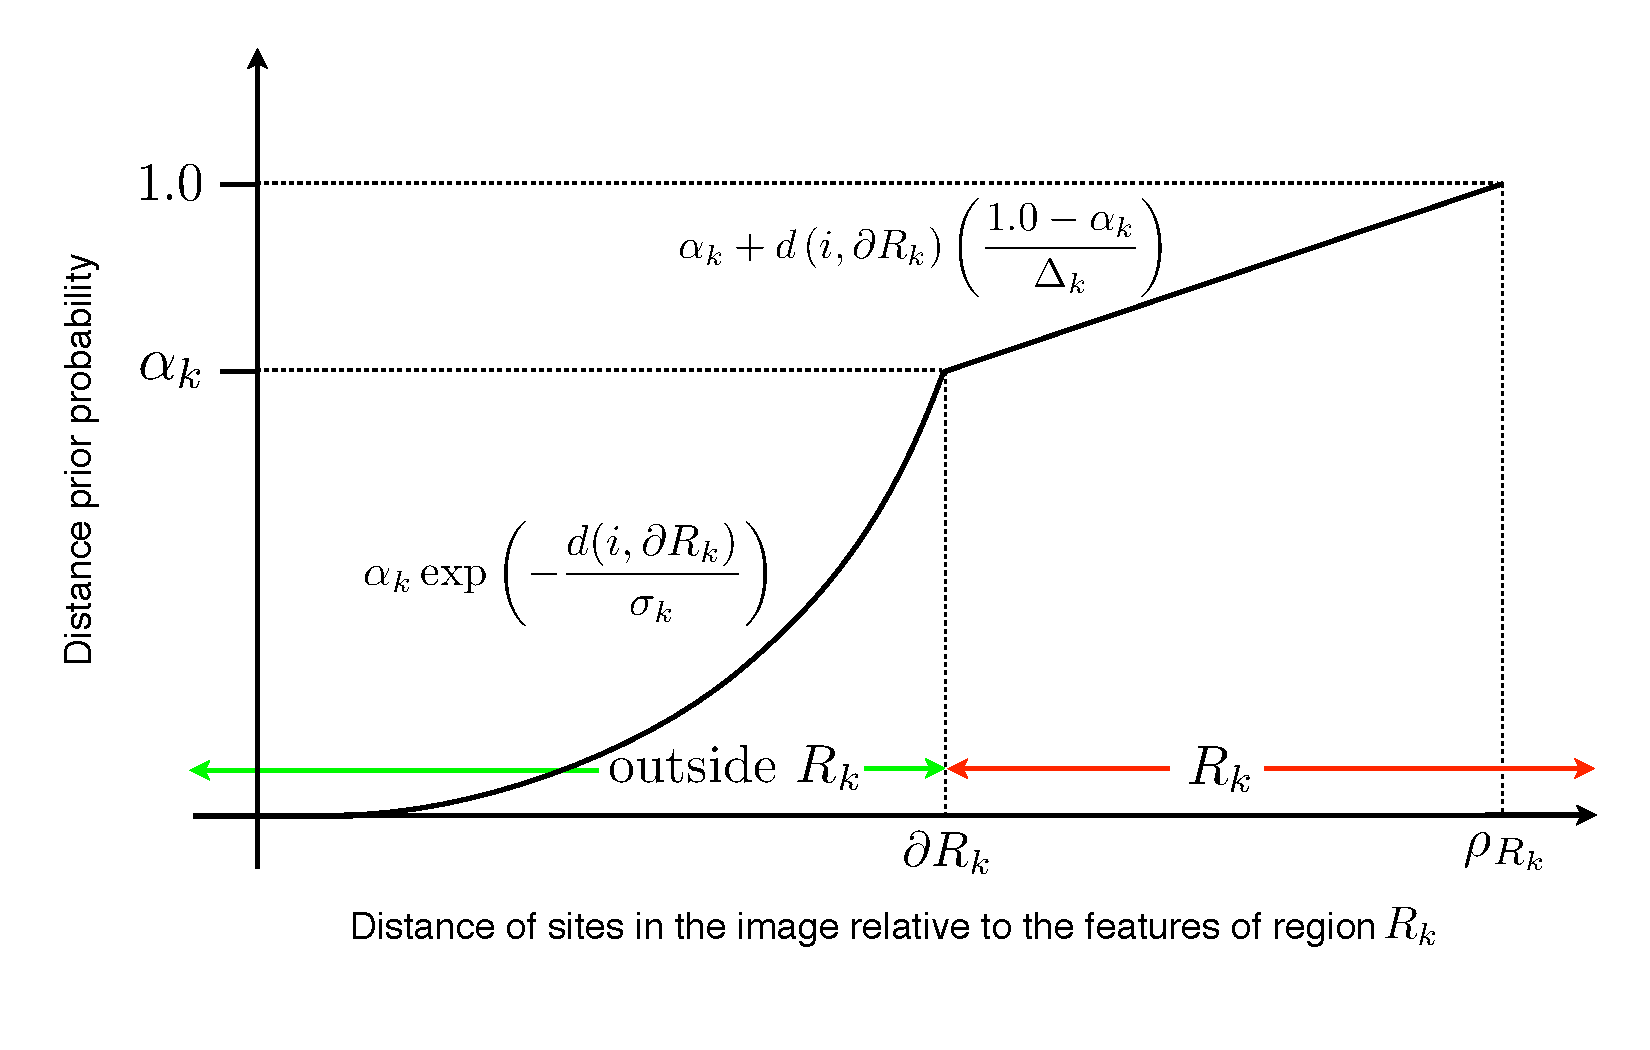
\includegraphics[width=150mm]{distancePrior.pdf}
\end{tabular}
\caption{\baselineskip 12pt \small Graphical representation of the distance prior probability calculation associated with label $l_k$.  This extension of the popular template-based prior probability strategy permits a dense labeling with the user specified mask. }
\label{fig:distancePrior}
\end{center}
\end{figure}



A crucial matter, particularly for propagating labels in the cortical
regions, is the choice of distance function.  One of the advantages to
surface-based methods is that distances can be calculated along the
surface mesh, thus discriminating between proximal cortical surface
points and those points which are situated close together due to
cortical folding.  In Atropos, we provide two possibilities---(1) a
geodesic distance function using a fast marching construction
\citep{Osher1988} of the distance function with Atropos's masked
region of interest and (2) a Euclidean distance function using the algorithm described in \cite{Maurer2003}.  The differences in label propagation results are illustrated in Fig.~\ref{fig:label_propagation}.   

Figure~\ref{fig:neonate} illustrates the benefit of geodesic distance
priors in segmenting T2 MRI of the 
neonatal brain.  Geodesic distance priors may be used to reduce ambiguity at
tissue interfaces, where partial voluming leads to mixed intensity.  
In neonatal brain segmentation from T2 MRI, the
interface of gray matter (low intensity) and cerebrospinal fluid
(bright intensity) often matches that of white matter (medium intensity). 
However, the white matter class should never appear near the surface
of the brain.  Thus, the distance from the brain surface may be used
to disambiguate voxels such as these.  
In this case, the distance of a voxel from a known
or expected tissue location serves to differentiate it from classes
that have similar intensity signature.  The geodesic distance is therefore an
alternative to explicit models of partial volume \citep{Ruan2000,Ballester2002,Leemput2003}. 

\begin{figure}
\begin{center}
\begin{tabular}{ccc}
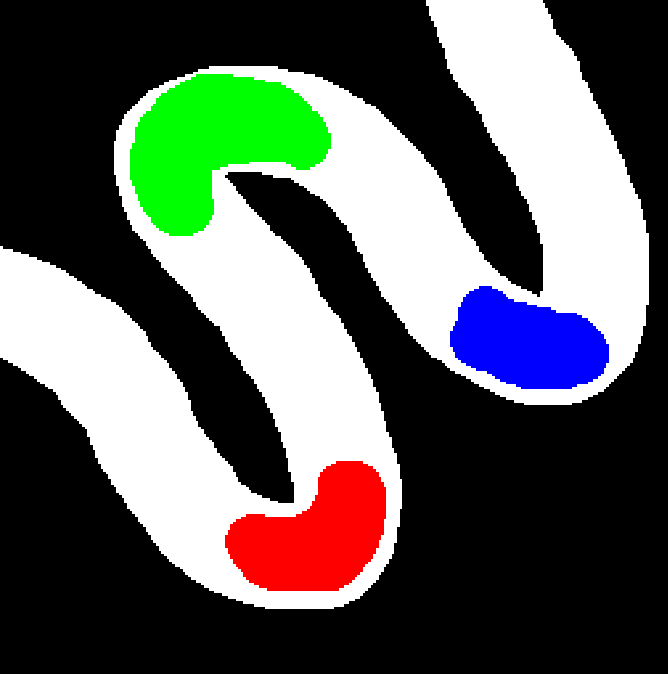
\includegraphics[width=50mm]{sparse_labels.png} &
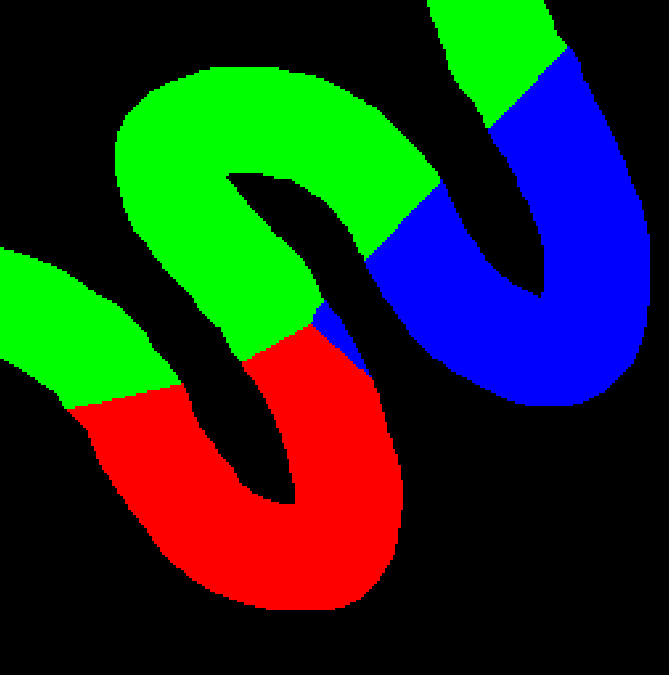
\includegraphics[width=50mm]{prop_euclidean.png} &
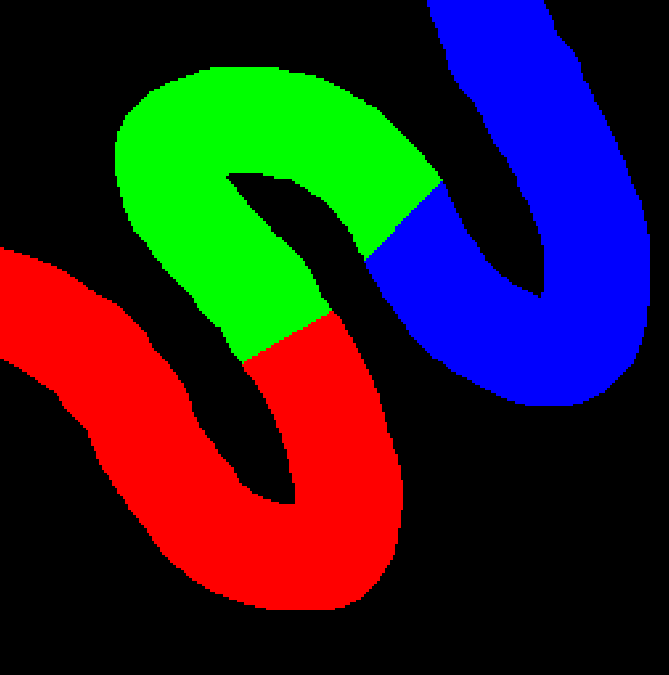
\includegraphics[width=50mm]{prop_geodesic.png} \\
(a) & (b) & (c) \\
\end{tabular}
\caption{\baselineskip 12pt \small  Illustration of label propagation differences between the Euclidean and geodesic approaches which
are particularly acute in sinuous structures such as the cortex.  (a) Given a mask, represented in white, and a sparse labeling,
Atropos can be used to propagate the labels in a dense manner throughout the masked region.  (b) This propagation can occur using Euclidean distances in the image space via an Euclidean distance transform which can cause labels to jump meaningful anatomical boundaries.   (c) Given the cortical geometry, a more intuitive approach would be to propagate the labelings in a geodesic manner using a product of the fast marching paradigm which can be used in a manner that respects anatomical boundaries.  }
\label{fig:label_propagation}
\end{center}
\end{figure}

\begin{figure}
\begin{center}
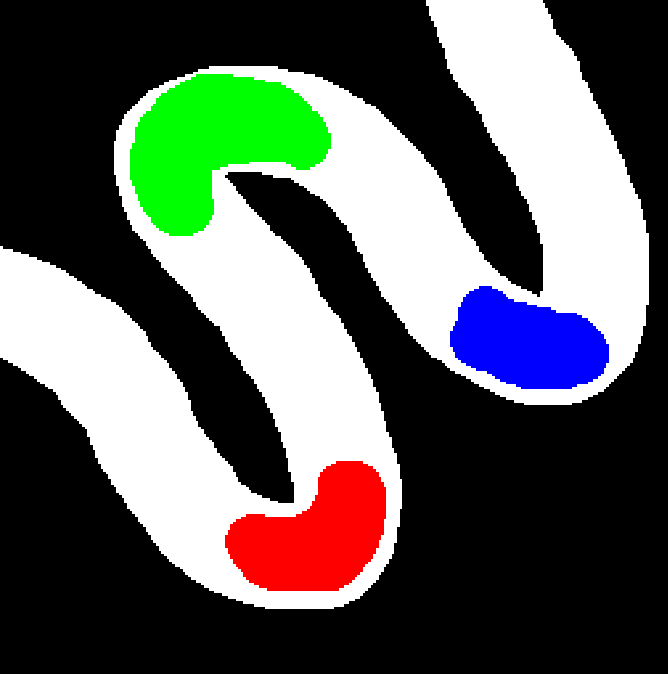
\includegraphics[width=0.9\textwidth]{sparse_labels.png} 
\caption{\baselineskip 12pt \small  Neonatal brain segmentation.  }
\label{fig:neonate}
\end{center}
\end{figure}


\subsection{Optimization}
Given the likelihood models and prior probabilities whose product is proportional to the posterior probability, the Bayesian segmentation solution is the labeling $\hat{\mathbf{x}}$ which maximizes the posterior probability, i.e.
\begin{align}
  \hat{\mathbf{x}} = \argmax_{\mathbf{x}} \left\{p(\mathbf{y}|\mathbf{x})p(\mathbf{x})\right\}.
\end{align}
Similar to its algorithmic predecessors, Atropos employs the EM
framework \citep{Dempster1977}.  After initial estimation of the
likelihood model parameters, EM iterates between calculation of the missing $\hat{\mathbf{x}}$ and subsequent re-estimation of the model parameters by maximizing the expectation of the complete data log-likelihood (cf. Eqn. (\ref{eq:likelihood})).
%\begin{align}
%\log( p(\mathbf{y}) ) = \sum_{i=1}^N \log \left( \sum_{k=1}^K \gamma_k  p(\mathbf{y}|l_k)  \right)
%\end{align}
The expectation maximization procedure is derived in various
publications including \cite{Zhang2001} which yields the optimal mean
and variance (or covariance), but sets the mixing parameter $\gamma_k$
as a constant.  The Atropos implementation estimates $\gamma_k$ at
each iteration as in \cite{Ashburner2005}.
\footnote{
Due to the lack of parameters in the non-parametric approach, it is not technically an EM algorithm (as described in \cite{Wells1996}).  However, the same iterative strategy is applicable and is quite robust in practice as evidenced by the number of researchers employing non-parametric strategies (see the Introduction).
}  
When spatial coherence constraints are included as an MRF prior in Atropos, the optimal segmentation solution becomes intractable.%
\footnote{
Consider $N$ sites each with a possible $K$ labels for a total of $N^K$ possible labeling configurations.  Due to the large $K$ associated with cortical labeling problems, exact optimization is even more problematic than for the traditional 3-tissue scenario.
}
Although many optimization techniques exist \citep[see the
introduction in][for a concise summary of the myriad optimization
possibilities]{Marroquin2002}---each with their characteristic
advantages and disadvantages in terms of computational complexity and
accuracy---Atropos uses the well-known {\em Iterated Conditional
  Modes} (ICM)  \citep{Besag1986} which is greedy, computationally efficient and provides good performance.

%\begin{align}
%P(l_k | y_i, t_i, m_i,d_i) &= \frac{P(y_i|l_k ,t_i,m_i,d_i)   P(l_k|t_i,m_i,d_i)   }{P(y_i|t_i,m_i,d_i)}
%\end{align}



%An image, $I$, maps a domain, $\Omega$ into the
%positive real numbers, such that $I \colon \Omega \rightarrow
%\mathbb{R}^+$.  The goal of segmentation, in general, is to define the
%spatial distribution of a finite set of labels over this domain.  We
%denote the segmentation itself as $\eta \colon \Omega \rightarrow L$
%where $L = \{ L_1 = 1 , \cdots , L_N=N \}$, a set of integer indexed
%segmentation labels.  Note that $\eta$ may be formed as $\eta =
%\sum_{i=1}^{i=N} L_i \eta_i $ where $\eta_i$ is the binary
%segmentation for label $L_i$.  A prior estimate for the label image
%$\eta_i$ is here denoted $\eta^s_i$ with a complete set of priors
%denoted $\eta^s$.  The boundary of the binary segmentation -- where a
%$0/1$ transition edge exists -- is denoted $\partial \eta^s_i$, for
%the prior, and $\partial \eta_i$ for the label image.
%
%\subsection{Apocrita Theory} A general maximum a posteriori criterion
%for segmentation seeks,
%\begin{equation} {\hat \eta} = \argmax _{\eta} \Pr( \eta | I )(\x) =
%\Pr( I | \eta )(\x) \Pr(\eta)(\x),
%\end{equation} 
%where $I$ is the input image, ${\eta}$ represents the
%label set configuration taken from the set $L$, $\Pr$ is the
%probability, $\x$ is the spatial index and the optimal solution is
%$\hat \eta$.  The input image $I$, here, is an unlabeled T1 MRI
%indexed by the value $\x \in \Omega$ where $\Omega$ is the image's
%spatial domain.  This probability is composed of the likelihood (first
%term) and the prior (second term).  Atropos ~ uses a spatially varying
%likelihood term and a two-component prior term that takes into account
%both spatial distribution and label smoothness, the latter via a
%standard MRF prior.
%
%The likelihood term for a single label value $L_i \in L$ is,
%\begin{eqnarray} \Pr( I | \eta_i )(\x)=\frac{1}{Z_i} \exp(- \| I(\x) -
%\mu_i(\x) \|^2 / \sigma_i^2 ),
%\end{eqnarray} where $Z_i$ is a normalizing constant, $\mu(\x)$ is a
%spatially varying estimate of the tissue mean and $\sigma$ is a
%standard deviation.  The prior term is given by,
%\begin{eqnarray} \Pr(\eta_i)(\x) = \frac{1}{Z^\prime_i} \exp( -f( \x -
%\y_{\partial \eta^s_i} ) / \sigma_{\eta^s_i}^2 ) p(\eta_i |
%\eta^\aleph_i), \\ \notag f( \x - \y_{\partial \eta^s_i} ) = (1 -
%\eta^s_i (\x) ) \| \x - \y_{\partial \eta^s_i} \|,
%\end{eqnarray} where $p(\eta_i | \eta^N_i)$ is the MRF smoothness
%probability based on the local neighborhood $\aleph$, the $Z$ is a
%normalizing constant and $\y_{\partial \eta^s_i}$ is the nearest point
%to $\x$ on the boundary of this labeling. Atropos ~requires a user or
%template-defined $\eta^s_i$ and the standard deviation
%$\sigma_{\eta^s_i}$ if a non-unity spatial prior component is desired
%for that label.  The free parameters, that must be estimated
%iteratively, are therefore $\mu_i, \sigma_i$ and the label set itself
%$\hat \eta$, which defines the (locally) optimal spatial distribution
%of $L$ through $\Omega$.  Figure~\ref{fig:spatp} shows the
%distribution of the spatial prior as a function of the distance from
%prior-defined object boundary.  Note that $f$ may easily be varied for
%other applications or that fixed probability images may also be
%substituted here.  This choice of $f$ is motivated by the fact that it
%allows compressed storage of the priors in a single image, $\eta^s$,
%while also maintaining the ability to manipulate -- for each
%$\eta^s_i$ -- the spatial influence of the prior via
%$\sigma_{\eta^s_i}$.  Practically, this is especially valuable when,
%$N$, the number of labels, is large.


\section{Implementation} 

\begin{figure}
\begin{center}
\begin{tabular}{c}
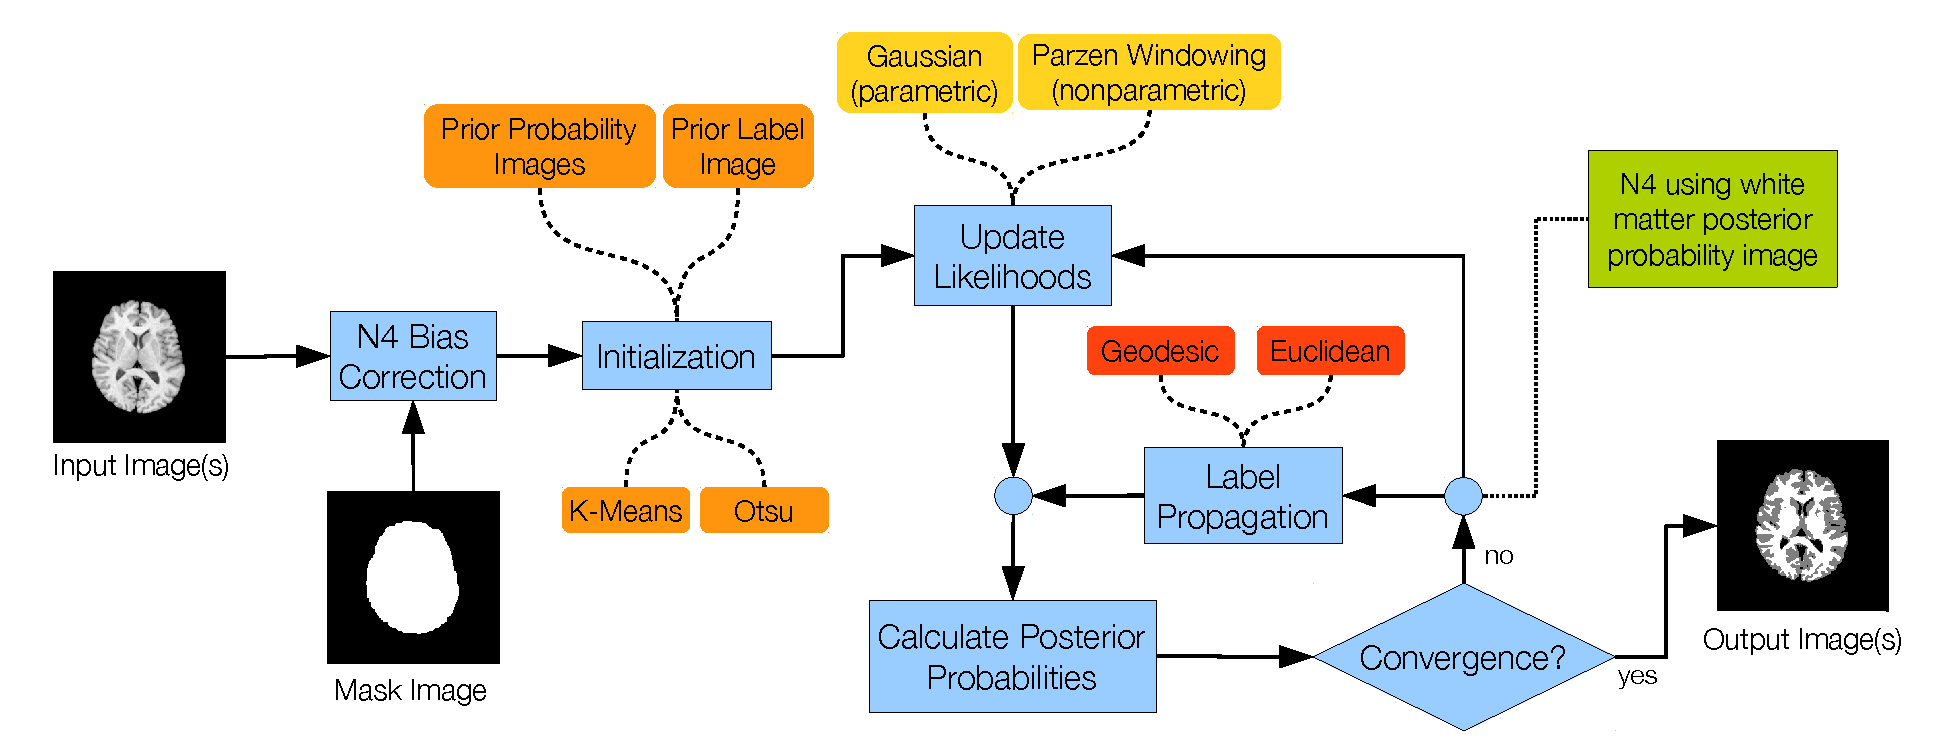
\includegraphics[width=160mm]{AtroposFlowchart.pdf}
\end{tabular}
\caption{\baselineskip 12pt \small Flowchart illustrating Atropos usage typically beginning with bias correction using the N4 algorithm.  
Initialization provides an estimate before the iterative segmentation portion of the algorithm in which the 
likelihood models for each class are tabulated from the current estimate followed by a recalculation of the 
posterior probabilities associated with each class.  Label propagation ensues to ensure a dense 
classification throughout the entire mask.   The multiple options associated with the different algorithmic 
components are indicated by the colored rounded rectangles connected to their respective core Atropos 
processes via curved dashed lines.  }
\label{fig:flowchart}
\end{center}
\end{figure}

As with other classes that comprise ANTs, Atropos uses the Insight Toolkit as a developmental foundation.  
This allows us to take advantage of the mature portions of ITK (e.g. image IO) and ensures the 
integrity of the ancillary processes such as those facilitated by the underlying statistical framework.  Although Atropos is 
publicly distributed with the rest of the ANTs package, we plan to contribute the Atropos segmentation
framework to the Insight Toolkit where it can be vetted and further
improved by other interested researchers. 
{\textcolor{red}{FIXME ---- should we save this for a deliverable in
    some grant?}}

An overview of the core components of Atropos can be gleaned, in part, from the flowchart depicted in 
Fig.~\ref{fig:flowchart}.  To provide a more intuitive interface without the overhead costs of a graphical user interface, a set of unique command line parsing classes were developed which can also provide insight to the functionality of Atropos.  
The short version of the command line help menu is given in Listing \ref{listing:command} which is invoked by typing `{\ttfamily Atropos -h}' at the command prompt.  Both short and long option flags are available and each option has its own set of possible values and parameters introduced in a more formal way in both previous discussion and related papers cited in the introduction.  Here we  describe these options from the unique perspective of  implementation.

\singlespacing 
\begin{command}
\lstsetcpp
\begin{lstlisting}
COMMAND: 
     Atropos

OPTIONS: 
     -d, --image-dimensionality 2/3/4
     -a, --intensity-image [intensityImage,<adaptiveSmoothingWeight>]
     -b, --bspline [<numberOfLevels=6>,<initialMeshResolution=1x1x...>,<splineOrder=3>]
     -i, --initialization Random[numberOfClasses]
                          KMeans[numberOfClasses]
                          Otsu[numberOfClasses]
                          PriorProbabilityImages[numberOfClasses,
                            fileSeriesFormat(index=1 to numberOfClasses) or vectorImage,
                            priorWeighting,<priorProbabilityThreshold>]
                          PriorLabelImage[numberOfClasses,labelImage,priorWeighting]
     -x, --mask-image maskImageFilename
     -c, --convergence [<numberOfIterations=5>,<convergenceThreshold=0.001>]
     -k, --likelihood-model Gaussian
                            HistogramParzenWindows[<sigma=1.0>,<numberOfBins=32>]
     -m, --mrf [<smoothingFactor=0.3>,<radius=1x1x...>]
     -o, --output [classifiedImage,<posteriorProbabilityImageFileNameFormat>]
     -u, --minimize-memory-usage (0)/1
     -w, --winsorize-outliers BoxPlot[<lowerPercentile=0.25>,<upperPercentile=0.75>,
                               <whiskerLength=1.5>]
                              GrubbsRosner[<significanceLevel=0.05>,<winsorizingLevel=0.10>]
     -e, --use-euclidean-distance (0)/1
     -l, --label-propagation whichLabel[sigma=0.0,<boundaryProbability=1.0>]
     -h 
     --help 
\end{lstlisting} 
\end{command}
\doublespacing 



\subsection{Integration of N4 Bias Correction}

The typical processing pipeline begins with an intensity normalization/bias correction
step using the recently developed N4 algorithm \citep{Tustison2010} which is based on the popular nonparametric 
nonuniformity intensity normalization (N3) method introduced in \cite{Sled1998}.    It was previously mentioned that several methods proposed in the literature have taken an integrative view of the segmentation problem by incorporating an intrinsic bias correction step into the actual algorithmic workflow.   The advancements
introduced with the N4 algorithm permit such an adaptive integration with Atropos.  
Recent demonstrations suggest improved white matter segmentation produces better gain field estimates using N3 
\citep{Boyes2008}.  Thus, when performing 3-tissue segmentation, we use the posterior probability map of white matter
at the current  iteration as a weighted mask for input to N4.  This is done by setting the `{\ttfamily --weight-image}' option on the N4 command line call (see Listing \ref{listing:n4}) to the posterior probability image corresponding to the white matter produced as output in the Atropos call, i.e. `{\ttfamily Atropos --output}'.


\singlespacing 
\begin{command}
\lstsetcppnfour
\begin{lstlisting}
COMMAND: 
     N4BiasFieldCorrection

OPTIONS: 
     -d, --image-dimensionality 2/3/4
     -i, --input-image inputImageFilename
     -x, --mask-image maskImageFilename
     -w, --weight-image weightImageFilename
     -s, --shrink-factor 1/2/3/4/...
     -c, --convergence [<numberOfIterations=50>,<convergenceThreshold=0.001>]
     -b, --bspline-fitting [splineDistance,<splineOrder=3>,<sigmoidAlpha=0.0>,
                           <sigmoidBeta=0.5>]
                           [initialMeshResolution,<splineOrder=3>,<sigmoidAlpha=0.0>,
                           <sigmoidBeta=0.5>]
     -t, --histogram-sharpening [<FWHM=0.15>,<wienerNoise=0.01>,<numberOfHistogramBins=200>]
     -o, --output [correctedImage,<biasField>]
     -h 
     --help 
\end{lstlisting} 
\end{command}
\doublespacing 


\subsection{From Segmentation Theory to Atropos Implementation}

\subsubsection{Initialization}
Atropos was designed to be dimensionally generic in the sense that the same code can be used to handle 2-, 3-, and 
even 4-dimensional image data.  Higher dimensions are possible although we have not yet encountered such 
application-specific need.  Multiple images (assumed to be of the same dimension, size, origin, etc.) can be specified 
on the command line using the `{\ttfamily -a/--intensity-image}' option for each image.  The first image specified on the 
command line is used to initialize the Random, Otsu, or K-means labeling with the latter initialization further
refined by incorporating the additional intensity images, i.e. an initial univariate K-means clustering is determined 
from the first intensity image which, along with the other images, provides the starting multivariate cluster centers for a 
follow-up multivariate K-means labeling.    

Much of the ANTs-based processing in our lab (including Atropos) takes advantage of template-building strategies 
\citep{Avants2010} which are also offered  in ANTs.  Since aligned prior probability images and prior label maps are often 
associated with such templates, Atropos can be initialized with these data with their influence regulated by a prior probability
weighting term.  Although prior label maps can be specified as a single multi-label image, prior probability data are often represented as
multiple scalar images with a single image corresponding to a particular label.  For relatively small classifications, such as 
the standard 3-tissue segmentation (i.e. white matter, gray matter, and cerebrospinal fluid), this does not typically present
computational complexities using modern hardware.  However, when considering dense cortical parcellations where the number
of labels can range upwards of 74 per hemisphere \citep{Destrieux2010}, the memory load can be prohibitive if all label images 
are loaded into run-time memory simultaneously.  A major part of
minimizing memory usage in Atropos,  which corresponds to the boolean
`{\ttfamily -u/--minimize-memory-usage}' option, is the sparse
representation of each of the prior probability images.  
Motivated by the observation that these spatial prior probability maps tend to be highly localized for large quantities of  
cortical labels, a threshold is specified on the command line (default = 0.0) and only those probability values which exceed 
that threshold are stored in the sparse representation.  During the course of optimization, the prior probability image for a
given label is reconstructed on the fly as needed.  {\textcolor{red}For the NIREP data used in this manuscript where the images are 
on the order of $300 \times 300 \times 256$ and 32 cortical labels, this typically shrinks run-time memory usage from a 
peak of 10+ GB to approximately 1.5 GB. --- FIXME }  
 
 \subsubsection{Likelihood or Observation Models}
As mentioned previously in the introduction, different groups have opted for different likelihood models which have included
either parametric, specifically Gaussian, or nonparametric variations.  However, these approaches are similar in that 
they require a list sample of intensity data from the input image(s) and a list of weighting values for each observation 
of the list sample from which the model is constructed.  
In general, one may query model probabilities by passing a given pixel's single intensity (for univariate segmentation) or multiple intensities (for multivariate
segmentation) to the modeling function, regardless of whether the
function is parameter or non-parametric.  These similarities permitted the creation of a generic plug-in architecture
where classes describing both parametric and nonparametric  observational models are all derived from an abstract 
list sample function class.   Three likelihood classes have been developed, one parametric and two nonparametric,
and are available for usage although one of the nonparametric classes is still in experimental development.  The plug-in architecture even permits mixing likelihood models with different classes during the same run for a hybrid parametric/non-parametric approach although this possibility has yet to be fully explored.

If the Gaussian likelihood model is chosen, the list sample of intensity values and 
corresponding weights comprised of the posterior probabilities are used to estimate the Gaussian model parameters, i.e.
the mean and variance.  For the non-parametric model, the list sample and posteriors are used
in a Parzen windowing scheme on a weighted histogram to estimate the
observational model  {\textcolor{red} cite Suyash}.  

\subsubsection{Prior Probability Models}
Consistent with our previous discussion, we offer both an MRF-based
prior probability for modeling spatial coherence and the possibility
of specifying a set of prior probability maps or a prior label map
with the latter extendable to creating a dense labeling.  To invoke
the MRF `{\ttfamily -m/--mrf}' option, one specifies the smoothing
factor (or the granularity parameter, $\beta$, given in
Eqn. (\ref{eq:U}), and the radius (in voxels) of the neighborhood
system using the vector notation `{\ttfamily 1x1x1}' for a
neighborhood radius of 1 in all 3 dimensions.  Note that this radius
prescribes an $L_\infty$  {\textcolor{red} FIXME should this be $L_2$?} distance and thus includes not just the face-connected neighboring voxels.

To propagate labels with the specification of prior probability images or a prior label image, one needs to select the distance function (set by the `{\ttfamily -e/--use-euclidean-distance}' boolean option) which, by default, is determined by the geodesic distance.  The user also needs to set the label propagation parameters for one or more of the classes.  This  includes both the boundary probability and the exponential decay parameter, respectively $\alpha_k$ and $\sigma_k$ in Eqn. (\ref{eq:prop}).  

{\bf FIXME Prior label image definition?}

\section{Evaluation}

We evaluate the $N$-class Atropos GMM-MRF model, which includes 
strong use of template-based spatial priors in order to initialize 
and guide the method into a consistent local minimum.
Atropos~encodes a family of segmentation techniques that may be
instantiated for different applications but here we evaluate only two of
the many possibilites. First, we perform an evaluation on the BrainWeb
dataset using both the standard T1 image with multiple bias and noise
levels and also the BrainWeb20 data, which varies the underlying
anatomy.  Second, we evaluate the use of Atropos in improving whole
brain parcellation and excercise its ability to efficiently solve {\em
  many class} expectation maximization problem.  We choose this
evaluation problem in part to illustrate the flexibility of Atropos
and also the benefits of the novel, efficient implementation that
allows many-class problems to be solved with low memory usage ($<$2GB
for a 68 class model on 1mm$^3$ brain data).  


\subsection{BrainWeb Evaluation}
\label{sec:bweb}
 BET2 \citep{Battaglini2008}
against openly available silver-standard datasets, the BrainWeb 20
(BW20) \citep{Aubert-Broche2006a} 


BW20 results show that by relying upon accurate, high-resolution
diffeomorphic image registration \citep{Avants2010}, Atropos~is capable
of reliably segmenting the BW20 whole head data into the brain
composed of separate tissue classes for muscle, skin, skull and bone
marrow as well as the standard three tissues, cerebrospinal fluid and
gray and white matter.  Atropos's three-tissue performance compares
favorably with the standard EM-MRF algorithm, FAST (~Atropos~gray matter
mean dice=0.9442, FAST=0.903,~Atropos~white matter mean dice=0.9475 and
FAST=0.949) \citep{Klauschen2009}.  The brain extraction component of
the solution compares favorably with BET2 (~Atropos~achieved mean $\pm$
s.d. of 0.9642 $\pm$ stdev: 0.0098 dice coefficient and BET2 achieved
0.9682 $\pm$ 0.0068 with an insignificant difference in performance
$p=0.1943$).  

\subsection{The Hammers Dataset Evaluation}
\label{sec:hammers}
We also provide, at the above location, multi-template
labeling results derived from the Hammers dataset by applying the
{\verb ants_multitemplate_labeling.sh } script to the 19 datasets at
\url{http://www.brain-development.org/} \citep{Hammers2003,Heckemann2006}.
Results are competitive with both \citep{Heckemann2006,Heckemann2010} 
though the latter appears to use a different label set.  The closest
comparison may be made with \citep{Heckemann2006}, which uses almost the
same label set, though with 30 datasets in total.  Our results only
incorporated the 19 currently available online. 

\begin{comment}
{
\subsection{Brain Web}

\subsection{The LPBA40 Dataset}  
\label{sec:lpba}
The LONI Probabilistic Brain Atlas data, LPBA40, \citep{Shattuck2008} was collected at the North Shore Long
Island Jewish Health System imaging center and is maintained at UCLA.
LPBA40 contains 40 images (20 male $+$ 20 female) from normal, healthy
ethnically diverse volunteers with average age of 29.2 $\pm$ 6.3
years.  Each subject underwent 3D SPGR MRI on a 1.5T GE system
resulting in $0.86 \times 0.86 \times 1.5 mm^3$ images.  Each MRI in
the LPBA40 dataset was manually labeled with 56 independent structures
at the UCLA Laboratory of Neuro Imaging (LONI).  The test-retest
reliability of the labeling, across raters, was reported as a minimum
Jaccard ratio of $0.697$ in the supramarginal gyrus to a maximum of
$0.966$ in the gyrus rectus.  A single labeling of each image is made
available to the public and used, here, as silver-standard data 
for both training and testing in our cross-validation scheme. 

\subsection{The NIREP Dataset}  
The non-rigid image registration evaluation project (NIREP
http://www.nirep.org/) is a resource of 16 high quality labeled brain
images at 1$mm^3$.  Each brain was labeled with 32 cortical regions
(16 on each hemisphere) and an additional class of other gray matter
tissue.  Regions vary in size from large (inferior temporal region) to
small (temporal pole, insula gyrus, frontal pole).  The main drawback
is a lack of inter-rater reliability numbers -- in particular because
visual inspection and comparison of labelings reveals a degree of
inconsistency in labeling of particular regions across subjects.
Nevertheless, the NIREP dataset is perhaps the highest quality
evaluation dataset currently available for the cortex. 

}
\end{comment}


\section{Discussion}

{\color{red}{{\em Elaborate after including the results.} 

A more general advantage which extends beyond the scope of the experimental 
evaluation section of this paper is the flexibility of the Atropos algorithm.   This includes 
not only $n$-tissue segmentation and dense volumetric cortical parcellation,
as reported in this work, but Atropos is also used in conjunction with our ANTs registration tools for robust
brain extraction which has reported good performance in comparison with other
popular, publicly available brain extraction tools \citep{Avants2010a}.  An additional successful
application area is that of ventilation-based segmentation of hyperpolarized helium-3 MRI
\citep{Tustison2010a}.}}


%\paragraph{Acknowledgments}
%{This work was supported in part by NIH ... }

\newpage

\bibliographystyle{neuroinformatics}
\bibliography{atropos} 

\end{document}

